\section{Execution}
\label{sec:execution}

To perform the experiment, a D8 laboratory diffractometer from Bruker-AXS is used.
The measurements themselves as well as drive control is being taken care of by the software XRD Command.
As explained, the X-rays are created in an X-ray tube and then hit the Göbel mirror, 
a mirror specifically created to parallelise X-rays, since the tube emits them evenly throughout every direction.
Then, the X-rays hit the sample and are reflected so that they can enter the detector. \\

This arrangement, however, has to be adjusted before the real measurement can be started.
In order to do that, a multitude of scans is performed as shown in \autoref{fig:scans}.

\begin{figure}[H]
    \centering
    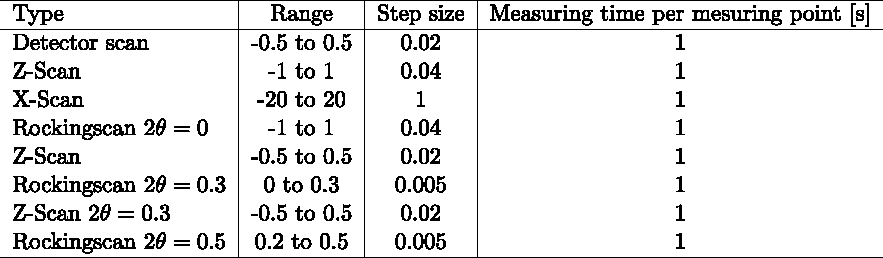
\includegraphics{figures/scans.pdf}
    \caption{A table showing the different scans that have to be performed in order to align the sample and the detector, 
    including the recommended settings for XRD Command \cite{v44}.}
    \label{fig:scans}
\end{figure}

As can be seen from the number of scans that need to be performed, it is important that the sample is aligned just right with the detector.
First the z-coordinate is aligned by moving the sample through the X-ray until it blocks half the intensity.
When adjusting the x-coordinate a plateau should show in the X-Scan.
the middle of the plateau is chosen and the sample is moved there via the diffractometer's drives.
The Rockingscans are performed to adjust the y-coordinate, which, as well as the Z-Scans, are performed multiple times at
different angles to ensure high precision. \\

After the alignment, the measurements are performed.
First, an \textbf{Omega/2Theta}-type scan with a range of $0°$ to $\SI{2.5}{\degree}$ and a step size of $\SI{0.005}{\degree}$ with $\SI{5}{\second}$ per step is performed.
Then, to measure the diffuse background, the detector is tilted by $\SI{0.2}{\degree}$ and the same measurement is performed again.


